\documentclass[a4paper]{article}

\usepackage{url}
\usepackage[MeX]{polski}
\usepackage[utf8]{inputenc}
\usepackage{lastpage}
\usepackage{fancyhdr}
\usepackage{graphicx}
\pagestyle{fancy}

\DeclareGraphicsExtensions{.pdf,.png,.jpg}
\graphicspath{{img/}}

\fancyhead{}
\fancyfoot{}

\lhead{Łukasz Buśko}
\rhead{\today}
\cfoot{\thepage\ of \pageref{LastPage}}

\begin{document}
\title{Dokumentacja \LaTeX \date{\today} }
\author{Łukasz Buśko\\
Licencja GPL\\
url{http://www.bedzie.jakas.pl} \\
email: buskol.waw.pl@gmail.com}

    \maketitle
%\cfoot{\thepage\ of \pageref{LastPage}}
    \newpage

    \tableofcontents
    \newpage

\section{Instalacja}
Pakiety wymagane do działania skryptu oraz kompilacji kernela:\\make, kernel-package, libncurses5-dev, fakeroot, wget, bzip2, build-essential\\
\verb # sudo apt-get -y install make kernel-package libncurses5-dev\\
\verb # sudo apt-get -y install fakeroot wget bzip2 build-essential\\
Można je też zainstalować automatycznie odpalając skrypt z parametrem:\\ \verb --install-packets
\\Skrypt działa z dowolnej lokalizacji pod warunkiem posiadania prawe wykonywania.\\
\verb # sudo chmod 111 dla możliwości wykonywania, przez każdego\\
bez możliwości ingerencji w sam skrypt \\
\verb # sudo chmod 600 config.conf, aby ustawienia dla naszego skryptu podlegały\\
tylko i wyłącznie nam.\\
\subsection{Skąd wziąć kernel?}
\begin{itemize}
\item Ubuntu - \verb http://kernel.debian.com/~kernel-ppa/mainline/
\end{itemize}

\newpage
\section{Konfiguracja}
Wszystkie zmienne skryptu, są przechowywane w pliku config.conf
\begin{itemize}
\item Sciezka - Ścieżka do katalogu ze źródłem *.deb.
\item Nazwa\verb _ kernela - Nazwa z jaka zostanie dodana do kernela.
\item specjalnaNazwaKernela - Nazwa dodatkowa pliku z własnoręcznie kompilowanym kernelem (Domyślnie Custom).
\item Log - Ścieżka do, w której zostanie utworzony plik logów.
\item KartaNV - Jeżeli posiadasz kartę Nvidii musisz ustawić wartość 1\\w przeciwnym wypadku wystąpi błąd instalacji kernela\\oraz karta nie będzie działać ze skompilowanym kernelem.
\end{itemize}
\begin{center}
\setlength\fboxsep{0pt}
\setlength\fboxrule{0.5pt}
\fbox{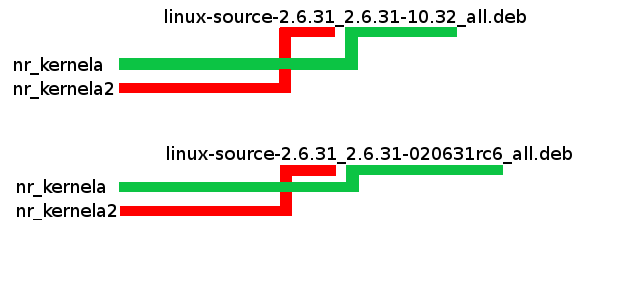
\includegraphics[scale=0.5]{instrukcja}}\begin{center}
\end{center}

\newpage
\section{Działanie}
\begin{flushleft}
Skrypt przeprowadzi rozpakowanie źródeł, skasuje nie potrzebne dane, skompiluje menu konfiguracyjne,\\
w którym własnoręcznie trzeba przeprowadzić optymalizacje.\\
Następnie skompiluje źródła kernela dokona instalacji. i skasuje zbędne pliki\\
po kompilacyjne\\
\end{flushleft}
\subsection{Parametry startowe}
\begin{itemize}
\item \verb --help,  \verb --h  - Wypisze pomoc i zakończy działanie.
\item \verb --version,  \verb --v -  Wypisze wersje i zakończy działanie.
\item \verb --compile-only,  \verb --c-o  - Dokonana zostanie jedynie kompilacja źródeł.
\item \verb --install-only,  \verb --i-o  - Zostanie przeprowadzona tylko instalacja już
\\skompilowanych źródeł.
\item \verb --install-packets,  \verb --i-p  - Zainstaluje pakiety potrzebne do przeprowadzenia kompilacji kernela.
\end{itemize}

\newpage
\section{Problemy}
\begin{itemize}
\item Po udanej instalacji programy wymagające prze kompilowania, zwracają komunikat /build does not exist
\\Oznacza to , że nie nagrałeś lub nagrałeś przed instalacja dodatkowy pakiet headerów.
\end{itemize} 

\newpage
\section{Błędy}
\begin{itemize}
\item
\end{itemize} 

\newpage
\section{Do zrobienia}
\begin{itemize}
\item
\end{itemize} 

\end{document}
